\subsection{Reconnaissance d'auteur}
\begin{frame}
	\frametitle{Auteur}
	\framesubtitle{Présentation du sujet}
	\paraTitle{Thème principal}
		\begin{itemize}
			\item Reconnaître l'auteur d'un texte
			\item Estimer le genre d'un auteur
		\end{itemize}
	
	\paraTitle{Plus-value possible}
		\begin{itemize}
			\item Peu (pas?) d'essais en Deep Learning.
			\item Peu d'essais en français.
		\end{itemize}

	\paraTitle{Applications possibles}
		\begin{itemize}
			\item Vérification de classification
			\item Analyse d'identité
			\item Validation auteur (cf. plagiat et/ou similarité)
		\end{itemize}
\end{frame}

\begin{frame}
	\frametitle{Auteur}
	\framesubtitle{Aspects techniques}
	\paraTitle{Bases de données}

		Extraitre de petites entités (paragraphes, tweets,...) via :
		\begin{itemize}
			\itemperso{Livres}Projet Gutenberg, Wikibooks,...
			\itemperso{Twitter}Récupération par API.
		\end{itemize}

	\paraTitle{Complexité}
		\begin{itemize}
			\item Problème ouvert
			\item Peu de sources		
		\end{itemize}
\end{frame}


\subsection{Inférence}
\begin{frame}
	\frametitle{Inférence}
	\framesubtitle{Présentation du sujet}
	\paraTitle{Thème principal}

		Extraire des relations entre phrases.
	
	\paraTitle{Plus-value possible}
		\begin{itemize}
			\item Peu d'essais en français.
			\item Comparaison entre langues.
		\end{itemize}

	\paraTitle{Applications possibles}
		\begin{itemize}
			\item Mise en avant de contradiction.
			\item Comparaison d'informations
		\end{itemize}
\end{frame}

\begin{frame}
	\frametitle{Inférence}
	\framesubtitle{Aspect technique}
	\paraTitle{Bases de données}
		\begin{itemize}
			\item Réutilisation de romans
			\item Articles de presse
			\item Stanford Natural Language Inference Corpus
		\end{itemize}

	\paraTitle{Complexité}
		\begin{itemize}
			\item Dépend de l'axe retenu
			\item Modélisation
			\item Grande variété de possibilités.
		\end{itemize}
\end{frame}

\subsection{Questions et réponses}
\begin{frame}
	\frametitle{Q\&A}
	\framesubtitle{Présentation du sujet}
	\paraTitle{Thème principal}
	
	Réponses automatiques à des questions simples.
	
	\paraTitle{Plus-value possible}
		\begin{itemize}
			\item Poursuivre les travaux en apprentissage par renforcement
		\end{itemize}

	\paraTitle{Applications possibles}
		\begin{itemize}
			\item Chatbox
			\item Proposition de services
		\end{itemize}
\end{frame}

\begin{frame}
	\frametitle{Q\&A}
	\framesubtitle{Aspects techniques}
	\paraTitle{Bases de données}
		\begin{itemize}
			\item Dialogues de films
			\item Autres difficiles à trouver (Facebook,...)
		\end{itemize}

	\paraTitle{Complexité}
		\begin{itemize}
			\item Utilisation de LSTM (technologie mature)
			\item Difficulté à trouver des BDDs 
			\item Difficulté de modélisation
			\item Manque de métrique pour évaluer
		\end{itemize}
\end{frame}

\subsection{Traduction}
\begin{frame}
	\frametitle{Traduction}
	\framesubtitle{Présentation du sujet}
	\paraTitle{Thème principal}

		Traduction à l'échelle d'un phrase par Deep Learning.
	
	\paraTitle{Plus-value possible}
		\begin{itemize}
			\item Un même réseau pour plusieurs langues.
			\item Trouver un autre cas d'usage?
		\end{itemize}
	
	\paraTitle{Applications possibles}

		Amélioration de résultats en traduction.
\end{frame}

\begin{frame}
	\frametitle{Traduction}
	\framesubtitle{Aspects techniques}
	\paraTitle{Bases de données}
	
		Tout ce qui est traduisible en plusieurs langues sur le web (cf. Linguee) :
		\begin{multicols}{2}
			\begin{itemize}
				\item Textes UE
				\item Brevets
				\item Documents légaux
				\item Site traduit
			\end{itemize}
		\end{multicols}

	\vspace*{-.2cm}

	\paraTitle{Complexité}
		\begin{itemize}
			\item Dépend de la précision
			\item Données présentes et technologies (LSTM) matures
		\end{itemize}
\end{frame}

\subsection{Analyse de sentiments}
\begin{frame}
	\frametitle{Sentiments}
	\framesubtitle{Présentation du sujet}
	\paraTitle{Thème principal}
		\begin{itemize}
			\item Classifier des phrases par sentiment.
			\item Prédire un sentiment (binaire ou avec une échelle).
		\end{itemize}

	\paraTitle{Plus-value possible}
		\begin{itemize}
			\item Combiner plusieurs approches.
			\item Problématique \og originale\fg.
		\end{itemize}

	\paraTitle{Applications possibles}
		\begin{itemize}
			\item Prendre le pouls de la \textit{twittosphère}.
			\item Classification de mails (injurieux ou non).
		\end{itemize}
\end{frame}

\begin{frame}
	\frametitle{Sentiments}
	\framesubtitle{Exemple d'arbre syntaxique}
	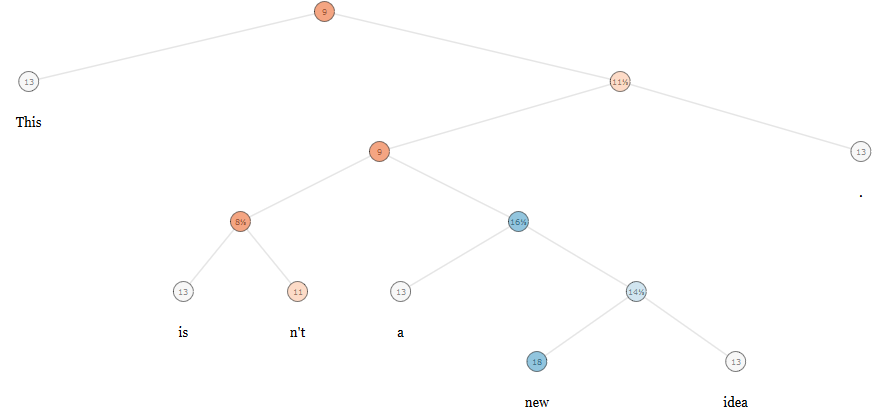
\includegraphics[width=\textwidth]{images/presentation/sampletree}
\end{frame}

\begin{frame}
	\frametitle{Sentiments}
	\framesubtitle{Aspects techniques}
	\paraTitle{Bases de données}
		\begin{itemize}
			\itemperso{IMDB, Amazon,...}Retours critiques de clients.
			\itemperso{Arbres syntaxiques}Stanford, 10000 arbres mais difficile à étendre (Amazon Turk).
		\end{itemize}

	\paraTitle{Complexité}
		\begin{itemize}
			\item Dépend de la précision et des outils.
			\item Base de données à aggréger.
			\item Grande variété de possibilités.
		\end{itemize}		
\end{frame}